\section{Scheduler for Distributed Execution}
\label{sec:schedule}


\noindent{\bf Issues.} The role of the scheduler is to consider the
constraint due to accessing a shared medium, so that only $k < n$
agents may broadcast their encoded messages. $k$ is
determined by the wireless communication environment. For example,
under a single wireless channel environment where each agent is
located in other agents' interference range, $k=1$.  Although the
number of agents that can be simultaneously scheduled is somewhat more
complex, we abstract it with a single number $k$ because the goal of
this paper lies in studying the importance of considering scheduling
constraints.

There are two key challenges in designing the scheduler: {\em (i)} how to
schedule agents in a distributed manner for decentralized execution, and
{\em (ii)} how to strike a good balance between simplicity in implementation
and training, and the integrity of reflecting the current practice of
MAC (Medium Access Control) protocols.

\begin{figure}[h!]
  \centering
  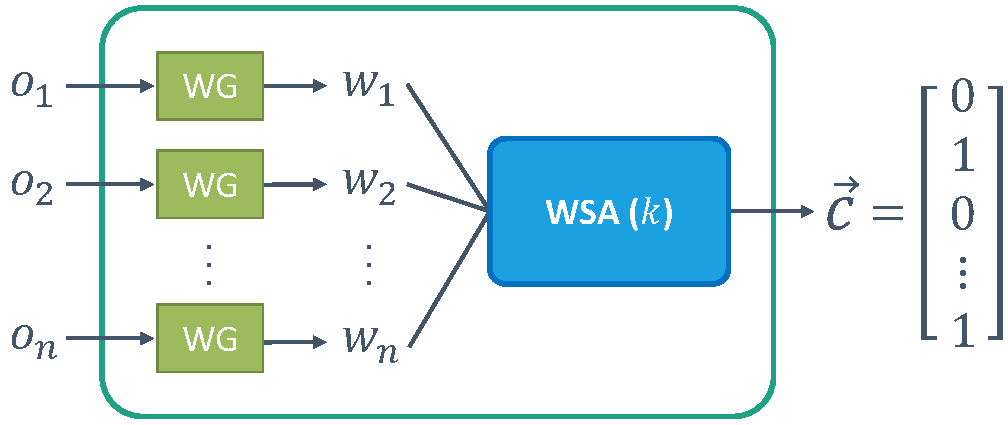
\includegraphics[width=0.5\columnwidth]{fig6}
  \vspace{-0.2cm}
\caption{\small Proposed scheduling architecture. 
  Each agent $i$ calculates its scheduling weight $w_i$
  from weight generator (WG), and
  the corresponding scheduling profile ${\bm c} \in \{0,1\}^n$
  is determined by the scheduling algorithm (k) (WSA(k)), satisfying the
  condition $||{\bm c}||_1 = k$.}

\label{fig:schedule_add}
\end{figure}

\paragraph{Weight-based scheduling}
To tackle the challenges addressed in the previous paragraph, we
propose a scheduler, called weight-based scheduler (WSA), that works based on each agent's individual weight
coming from its observation. As
shown in Figure~\ref{fig:schedule_add}, the role of WSA is to map from
$\vec{w}=[w_i]_n$ to $\vec{c}.$ This scheduling is extremely simple,
but more importantly, highly amenable to the philosophy of distributed
execution. The remaining checkpoint is whether this principle is
capable of efficiently approximating practical wireless scheduling
protocols. To this end, we consider the following two weight-based
scheduling algorithms among many different protocols that could be
devised:
\begin{compactitem}[$\circ$]

\item {\em Top($k$).} Selecting top $k$ agents in terms of their weight values. 

\item {\em Softmax($k$).} Computing softmax values $\sigma({\bm w})_i = \frac{e^{w_i}}{\sum_{j=1}^{n}e^{w_j}}$ for each agent $i,$ and then randomly selecting  $k$ agents with probability in proportion to their softmax values. 
\end{compactitem}

Top($k$) can be a nice abstraction of
the MaxWeight~\citep{tassiulas1992stability} scheduling principle or its
distributed approximation \citep{yy_scheduling}, in which case it is
known that different choices of weight values result in achieving
different performance metrics, {\em e.g.}, using the amount of messages
queued for being transmitted as weight. Softmax($k$) can be a
simplified model of CSMA (Carrier Sense Multiple Access), which forms
a basis of 802.11 Wi-Fi.  Due to space limitation, we refer the reader
to \citet{jiang2010distributed} for detail. We now present how {\em
  Top($k$)} and {\em Softmax($k$)} work.
 

\subsection{Carrier Sense Multiple Access (CSMA)}
CSMA is the one of typical distributed MAC scheduling in wireless
communication system. To show the feasibility of scheduling {\em
  Top($k$)} and {\em Softmax($k$)} in a distributed manner, we will
explain the variant of CSMA. In this section, we first present the
concept of CSMA.

\myparagraph{How does CSMA work?} The key idea of CSMA is ``listen
before transmit''. Under a CSMA algorithm, prior to trying to transmit
a packet, senders first check whether the medium is busy or idle, and
then transmit the packet only when the medium is sensed as idle, {\em i.e.}, no
one is using the channel. To control the aggressiveness of such medium
access, each sender maintains a backoff timer, which is set to a
certain value based on a pre-defined rule. The timer runs only when
the medium is idle, and stops otherwise. With the backoff timer, links
try to avoid collisions by the following procedure:
\begin{itemize}
\item Each sender does not start transmission immediately when the
  medium is sensed idle, but keeps silent until its backoff timer
  expires.
\item After a sender grabs the channel, it holds the channel for some
  duration, called the holding time.
\end{itemize}
Depending on how to choose the backoff and holding times, there can be
many variants of CSMA that work for various purposes such as fairness
and throughput. Two examples of these, {\em Top($k$)}
and {\em Softmax($k$)}, are introduced in the following sections.


\subsection{A version of {\em Distributed Top($k$)} }
In this subsection, we introduce a simple distributed scheduling
algorithm, called {\em Distributed Top($k$)}, which can work with
\sched -Top($k$). It is based on CSMA where each sender determines
backoff and holding times as follows.  In \sched, each agent generates
the scheduling weight $w$ based on its own observation. The agent sets its
backoff time as $1-w$ where $w$ is its schedule weight, and it waits
for backoff time before it tries to broadcast its message. Once it
successfully broadcasts the message, it immediately releases the channel.
Thus, the agent with the highest $w$ can grab the channel in a
decentralized manner without any message passing. By repeating this
for $k$ times, we can realize decentralized Top($k$) scheduling.

To show the feasibility of distributed scheduling, we implemented the
Distributed Top($k$) on Contiki network simulator~\citep{contiki} and
run the trained agents for the PP task. In our experiment, Top($k$) agents
are successfully scheduled 98\% of the time, and the 2\% failures are
due to probabilistic collisions in which one of the colliding agents is
randomly scheduled by the default collision avoidance mechanism implemented in
Contiki. In this case, agents achieve 98.9\% performance compared to
the case where Top($k$) agents are ideally scheduled.

\subsection{oCSMA Algorithm and {\em Softmax($k$)}}
In this section, we explain the relation between {\em Softmax($k$)} and
the existing CSMA-based wireless MAC protocols, called oCSMA. When we
use {\em Softmax($k$)} in the case of $k = 1$, the scheduling
algorithm directly relates to the channel selection probability of
oCSMA algorithms. First, we explain how it works and show that the
resulting channel access probability has a same form with {\em
  Softmax($k$)}.

\myparagraph{How does oCSMA work?} It is also based on the basic CSMA
algorithm. Once each agent generates its scheduling weight $w_i$, it sets
$b_i$ and $h_i$ to satisfy $w_i = \log(b_i h_i)$. It sets its backoff
and holding times following exponential distributions with means
$1/b_i$ and $h_i$, respectively. Based on these backoff and holding
times, each agent runs the oCSMA algorithm. In this case, if all agents are
in the communication range, the probability that agent $i$ is
scheduled over time is as follows:
$$s_i (\bm{w}) 
= \frac{\exp(w_i)}{\sum_{j=1}^{n} \exp(w_j)}.$$
 We refer the readers to \citet{jang} for detail.

\begin{comment}

 \note{DW: I think it would be better to remove below} \vspace{3cm}






\myparagraph{Wireless network model} In a wireless network, links
sharing the wireless medium has a interference effect with each
other. This interference relation can be modeled as a graph
$\mathcal{G} = (\mathcal{L}, \mathcal{E})$ where $\mathcal{L}$ and
$\mathcal{E}$ denotes the set of links and edges between interfering
links, respectively.  We define a scheduling vector as
$\bm{\sigma} \triangleq \{ \sigma_i : i \in \mathcal{L} \} $ where
$\sigma_i \in \{0,1\}$ and $\sigma_i = 1$ means the link $i$ is
scheduled for transmission.  We call a schedule $\bm{\sigma}$ is
feasible if there exists no edges $(i, j) \in \mathcal{E}$ where
$\sigma_i + \sigma_j > 1$, i.e., link $i$ and link $j$ is scheduled at
a same time.  Formally, the set of all feasible schedules
$\mathcal{I}(\mathcal{G})$ is defined as
$$\mathcal{I}(\mathcal{G}) \triangleq \{ \bm{\sigma} \in \{ 0, 1 \} ^n :
 \sigma_i + \sigma_j \leq 1 , \forall (i, j) \in \mathcal{E} \}.$$
In the environment given to \sched~with $k = 1$, the interference graph
$\mathcal{G}$ is a complete graph, i.e., $(i, j) \in \mathcal{E}$ for all
pairs of $i \neq j$ in $\mathcal{L}$. Also the ``link'' mentioned
in this section refers to the ``agent'' in \sched~setting.

\myparagraph{Analysis of oCSMA}
An oCSMA algorithm described above induces a sequence of schedules
$\{\bm{\sigma} (t)\}_{t=0}^{\infty}$, which is a time-reversible,
continuous-time Markov process. To illustrate, consider a simple
three-link interference graph and its resulting Markov process in
Figure~\ref{fig:three}.



\begin{figure}[ht!]
\centering   
\includegraphics[width=0.6\columnwidth]{fig/3link_MC_fig}
\caption{\small (a) 3-link interference graph, where links 1 and 3 do not
    interfere with each other, but interfere
    only with link 2. (b) The resulting CSMA Markov process for fixed
    intensities, where for example the state $(1,0,1)$ means that links
    1 and 3 are active and link 2 is inactive.}
\label{fig:three}
\end{figure}

For fixed CSMA parameters $\bm{b} = [b_i]_{i \in \mathcal{L}}$ and
$\bm{h} = [h_i]_{i \in \mathcal{L}}$, using the time-reversibility of
Markov process $\{\bm{\sigma} (t)\}_{t=0}^{\infty}$, its stationary
distribution $\pi^{\bm{b},\bm{h}} = 
[\pi^{\bm{b},\bm{h}}_{\bm{\sigma}}]_{\bm{\sigma} \in \mathcal{I}(\mathcal{G})}$
is characterized as
$$\pi_{\bm{\sigma}}^{\bm{b},\bm{h}}= \frac{\prod_{i \in \mathcal{L}} (b_i h_i)^{\sigma_i}}{\sum_{\bm{\sigma'} \in \mathcal{I}(\mathcal{G})} \prod_{i \in \mathcal{L}} (b_i h_i)^{\sigma'_i}}.$$
Namely, the stationary distribution of a schedule depends only on the
product of $\bm{b}$ and $\bm{h}$ of links.  For simple presentation,
we let $r_i = \log(b_i h_i)$ and $\bm{r} = [r_i]_{i \in \mathcal{L}}$,
and call $r_i$ the {\em intensity} of link $i,$ intuitively meaning
the transmission aggressiveness of the link. In the above explanation
of oCSMA, we set $r_i$ as the scehduling weight $w_i$.  We also use
$\pi^{\bm{r}}$ instead of $\pi^{\bm{b},\bm{h}}$.

Given the links' fixed intensities $\bm{r}$, the ergodicity of the
Markov process implies that the marginal probability
$s_i(\bm{r}) \triangleq P(\sigma_i (t) = 1 | \bm{r})$ that link $i$ is
scheduled under the stationary distribution $\pi^{\bm{r}}$ becomes the
link $i$'s long-term (average) throughput or service rate, \ie,
$\lim_{t\to\infty} \frac1t \int^{t}_{0}\sigma_i(s)\,ds$.  Furthermore,
using the reversibility of the Markov process, the marginal
probability can be characterized as:
\begin{eqnarray} \label{eq:throughput}
s_i(\bm{r}) = \mathbb{E}_{\pi^{\bm{r}}}[\sigma_i] = \sum\limits_{\bm{\sigma} \in \mathcal{I}(\mathcal{G}): \sigma_i=1} \pi_{\bm{\sigma}}^{\bm{r}}
= \frac{\sum_{\bm{\sigma} \in \mathcal{I}(\mathcal{G})|\sigma_i = 1} \exp(\sum_{i \in \mathcal{L}} \sigma_i r_i)}{\sum_{\bm{\sigma'} \in \mathcal{I}(\mathcal{G})} \exp(\sum_{i \in \mathcal{L}} \sigma'_i r_i)}.
\end{eqnarray}

\myparagraph{How {\em Softmax($k$)} and CSMA are connected}
So far we discussed about the stationary distribution of a Markov process
induced by CSMA algorithms under a general interference graph $\mathcal{G}$.
However, as said earlier, the interference graph given by our environment
is a complete graph. The set of all feasible schedules $\mathcal{I}(\mathcal{G})$
is given as
$$\mathcal{I}(\mathcal{G}) = \{ \bm{\sigma} \in \{0,1\}^n : ||\bm{\sigma}||_1 = 1 \}.$$
Deonte $\bm{\sigma}^i$ as a one-hot vector where only $i$-th element is one.
Then equation (\ref{eq:throughput}) is reduced as
$$s_i (\bm{r}) = \frac{\sum_{\bm{\sigma} \in \mathcal{I}(\mathcal{G})|\sigma_i = 1} \exp(\sum_{i \in \mathcal{L}} \sigma_i r_i)}{\sum_{\bm{\sigma'} \in \mathcal{I}(\mathcal{G})} \exp(\sum_{i \in \mathcal{L}} \sigma'_i r_i)}
 = \frac{\exp(r_i)}{\sum_{\bm{\sigma}^j} \exp(r_j)}
 = \frac{\exp(r_i)}{\sum_{j=1}^{n} \exp(r_j)}.$$
Therefore, we can say the marginal channel access probability induced by
CSMA algorithm is same as {\em softmax(1)}.

\end{comment}

%%% Local Variables:
%%% mode: latex
%%% TeX-master: "main"
%%% End:
